An experiment was conducted where a test sample was additively manufactured with purposely designed voids. The objective is to see if the voids can be detected using a single projection. This was done by comparing a projection of the test sample with the simulation of that projection as if the voids were not there. The simulated projections were produced by software called \emph{aRTist} \citep{bellon2007artist, jaenisch2008artist, bellon2012radiographic}. It can simulate projections of the test sample given the specifications of the CT apparatus, such as the x-ray source and the x-ray detector, and the CAD of the test sample \citep{bellon2011simulation, deresch2012simulating}.

\cite{brierley2018optimized} did something similar by comparing a projection of the test sample, with no voids, with a simulation of that projection with voids added. The experiment presented here is the other side of the coin, putting voids in the physical test sample rather than in the simulated projection. This makes the experiment more realistic by attempting to detect real voids. Being able to detect voids suggest quality control can be done in projection space, rather than reconstruction space, to speed up the quality control procedure.

This chapter describes the apparatus used to manufacture the test sample and obtaining the projections. There is also a discussion, at the end of the chapter, on shading correction which was used to remove detector panel and x-ray spot effects from the projections.

Many figures presented here were given by engineers in relation to the experiment or by the manufacturer. Figures with no error bars were rounded to an appropriate number of significant figures.

\section{Apparatus}

The test object is a cuboid (\SI{40.0}{\milli\metre} $\times$ \SI{40.0}{\milli\metre} $\times$ \SI{60.0}{\milli\metre}) with voids, the CAD shown in Figure \ref{fig:inference_testObject}. The voids were of diameters \SI{2.4}{\milli\metre}, \SI{1.2}{\milli\metre}, \SI{0.6}{\milli\metre} and \SI{0.3}{\milli\metre}. 6 voids for each diameter were designed in the CAD. Voids with diameters \SI{2.4}{\milli\metre} and \SI{0.6}{\milli\metre} were regularly arranged, otherwise they were arranged irregularly.

\begin{figure}
  \centering
  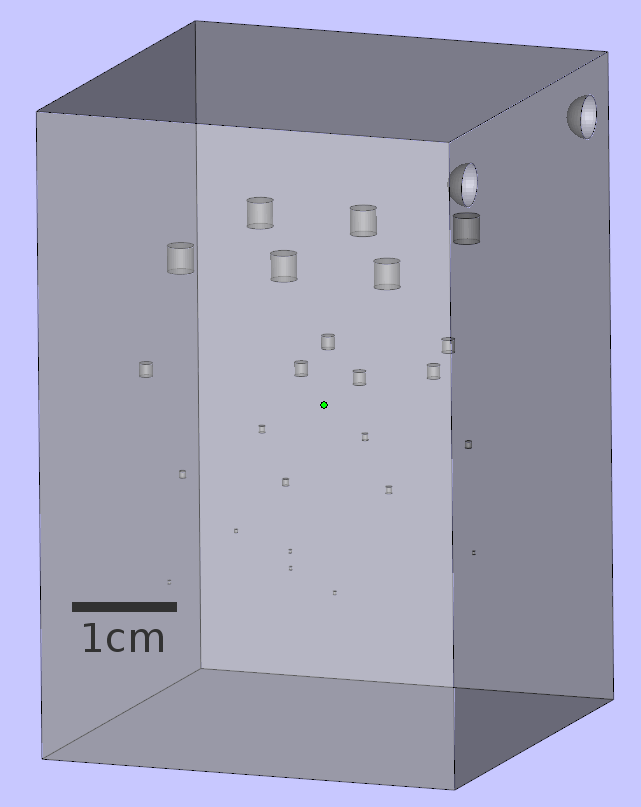
\includegraphics[width=0.4\textwidth]{../figures/inference/TestObject.png}
  \caption{CAD of the test object; the scale shown is approximate.}
  \label{fig:inference_testObject}
\end{figure}

The \emph{Fortus 400mc (Stratasys, US)} was used to manufacture the test object made of plastic (acrylonitrile butadiene styrene or ABS). The precision of the manufacturing was in the order of $\pm\SI{0.1}{\milli\metre}$ \citep{hanseen2013fortus}. Another test object was manufactured made from titanium (Ti-6Al-4V)

X-ray projections were obtained using the \emph{Nikon XT H LC 225/320} x-ray CT scanner (\emph{Nikon Metrology, UK}) together with a \emph{Perkin Elmer XRD 1621 (Perkin Elmer, US)} detector. The target material in the x-ray source is tungsten. The sensor in the detector is made up of 2 rows and 16 columns of panels. The sensor has dimensions of $\SI{409.6}{\milli\metre}\times\SI{409.6}{\milli\metre}$ which produced a projection of $\SI{2048}{\pixel}\times\SI{2048}{\pixel}$ in size \citep{perkinelmer2006xrd}. Therefore the scale of each pixel is $\SI{200.0}{\micro\metre\per\pixel}$. The projections were cropped to $\SI{2000}{\pixel}\times\SI{2000}{\pixel}$ to remove boundary effects. The gain and offset were adjusted by the engineers to produce a projection with good contrast, each pixel then has a grey value in units of analogue to digital units (\SI{}{\adu}).

Greyscale projections were taken in addition to the projection of the test object. These are projections with nothing between the source and the detector with the x-ray tube at different powers. The power was varied by fixing the potential difference and varying the current. The greyscale projections were used for calibration such as shading correction. The greyscale projection with the x-ray turned off is called the black image. The greyscale projection with the x-ray set up the same when obtaining the test object projection is called the white image.

Replicate test object projections and greyscale projections were obtained by repeating the acquisition. These replicated projections were used to study the noise observed in the projections.

Filters used to tackle beam hardening were used such as \SI{0.350}{\milli\metre} of copper and \SI{2.000}{\milli\metre} of tin.

\emph{aRTist} was used to simulate the test object projection and all greyscale projections except for the black image. The black image was simulated by producing an uniform image with grey value the mean over the obtained black image. The engineers used numerical methods to align the simulated projection with the obtained projection.

\section{Datasets}

3 datasets were collected and named \texttt{AbsNoFilter}, \texttt{AbsFilter} and \texttt{TiFilter}. Projections of the ABS test object were taken in \texttt{AbsNoFilter} and \texttt{AbsFilter}, the titanium test object was used in \texttt{TiFilter}. 2 angular projections were taken for all datasets. Greyscale projections were obtained as well. To investigate the effects of beam hardening, no x-ray filter was used in \texttt{AbsNoFilter}, a filter was used in \texttt{AbsFilter}.

The properties of each dataset is shown in Table \ref{table:data_dataset}. Properties include the x-ray tube, the XCT apparatus and what powers were used in the greyscale projections. A sample of the obtained, simulated and greyscale projections for the datasets \texttt{AbsNoFilter}, \texttt{AbsFilter} and \texttt{TiFilter} are shown in Figures \ref{fig:data_AbsNoFilter}, \ref{fig:data_AbsFilter} and \ref{fig:data_TiFilter} respectively.

\begin{sidewaystable}
\centering
\begin{tabular}{l|lll}
                                                       & \multicolumn{3}{c}{Dataset name}                                                \\
                                                       & \texttt{AbsNoFilter} & \texttt{AbsFilter}             & \texttt{TiFilter}        \\ \hline
potential difference (\SI{}{\kilo\volt})               & 80                   & 80                             & 190                      \\
power (\SI{}{\watt})                                   & 36                   & 20                             & 19.95                    \\
filter                                                 & no filter            & \SI{0.35}{\milli\metre} copper & \SI{3}{\milli\metre} tin \\
time exposure (\SI{}{\milli\second})                   & 708                  & 500                            & 1415                     \\
distance from source to object (\SI{}{\milli\metre})   & 217                  & 168                            & 86                       \\
distance from source to detector (\SI{}{\milli\metre}) & 1178                 & 876                            & 875                      \\
number of replications                                 & 100                  & 20                             & 20                       \\ \hline
powers used for greyscale projections (\SI{}{\watt})   & 0                    & 0                              & 0                        \\
\multicolumn{1}{c|}{\vdots}                            & 10.08                & 4.96                           & 10.07                    \\
\multicolumn{1}{c|}{\vdots}                            & 18.08                & 10                             & 19.95                    \\
\multicolumn{1}{c|}{\vdots}                            & 28                   & 15.04                          &                          \\
\multicolumn{1}{c|}{\vdots}                            & 36                   & 20                             &                          \\
number of replications                                 & 20                   & 20                             & 20                      
\end{tabular}
\caption{Properties of the 3 datasets obtained for the experiment.}
\label{table:data_dataset}
\end{sidewaystable}

\begin{figure}[p]
  \centering
  \centerline{
    \begin{subfigure}[b]{0.49\textwidth}
      \includegraphics[width=\textwidth]{../figures/data/AbsNoFilterDeg30.eps}
      \caption{Projection of sample at \SI{36}{\watt}}
    \end{subfigure}
    \begin{subfigure}[b]{0.49\textwidth}
      \includegraphics[width=\textwidth]{../figures/data/AbsNoFilterDeg30_sim.eps}
      \caption{Simulation of sample at \SI{36}{\watt}}
    \end{subfigure}
  }
  \centerline{
    \begin{subfigure}[b]{0.49\textwidth}
      \includegraphics[width=\textwidth]{../figures/data/AbsNoFilter_calibration1.eps}
      \caption{Projection at \SI{0}{\watt}}
    \end{subfigure}
    \begin{subfigure}[b]{0.49\textwidth}
      \includegraphics[width=\textwidth]{../figures/data/AbsNoFilter_calibration5.eps}
      \caption{Projection at \SI{36}{\watt}}
    \end{subfigure}
  }
  \caption{\texttt{AbsNoFilter} projections obtained; note the colour scale may vary.}
  \label{fig:data_AbsNoFilter}
\end{figure}

\begin{figure}[p]
  \centering
  \centerline{
    \begin{subfigure}[b]{0.49\textwidth}
      \includegraphics[width=\textwidth]{../figures/data/AbsFilterDeg30.eps}
      \caption{Projection of sample at \SI{20}{\watt}}
    \end{subfigure}
    \begin{subfigure}[b]{0.49\textwidth}
      \includegraphics[width=\textwidth]{../figures/data/AbsFilterDeg30_sim.eps}
      \caption{Simulation of sample at \SI{20}{\watt}}
    \end{subfigure}
  }
  \centerline{
    \begin{subfigure}[b]{0.49\textwidth}
      \includegraphics[width=\textwidth]{../figures/data/AbsFilter_calibration1.eps}
      \caption{Projection at \SI{0}{\watt}}
    \end{subfigure}
    \begin{subfigure}[b]{0.49\textwidth}
      \includegraphics[width=\textwidth]{../figures/data/AbsFilter_calibration5.eps}
      \caption{Projection at \SI{20}{\watt}}
    \end{subfigure}
  }
  \caption{\texttt{AbsFilter} projections obtained; note the colour scale may vary.}
  \label{fig:data_AbsFilter}
\end{figure}

\begin{figure}[p]
  \centering
  \centerline{
    \begin{subfigure}[b]{0.49\textwidth}
      \includegraphics[width=\textwidth]{../figures/data/TiFilterDeg30.eps}
      \caption{Projection of sample at \SI{20}{\watt}}
    \end{subfigure}
    \begin{subfigure}[b]{0.49\textwidth}
      \includegraphics[width=\textwidth]{../figures/data/TiFilterDeg30_sim.eps}
      \caption{Simulation of sample at \SI{20}{\watt}}
    \end{subfigure}
  }
  \centerline{
    \begin{subfigure}[b]{0.49\textwidth}
      \includegraphics[width=\textwidth]{../figures/data/TiFilter_calibration1.eps}
      \caption{Projection at \SI{0}{\watt}}
    \end{subfigure}
    \begin{subfigure}[b]{0.49\textwidth}
      \includegraphics[width=\textwidth]{../figures/data/TiFilter_calibration3.eps}
      \caption{Projection at \SI{20}{\watt}}
    \end{subfigure}
  }
  \caption{\texttt{TiFilter} Projections obtained; note the colour scale may vary.}
  \label{fig:data_TiFilter}
\end{figure}

The projections do indeed show the test sample, however, with panel and spot effects. The structure of the 32 panels are predominate in the black image in particular, this was observed by \cite{yang2009evaluation} as well. This is concerning because systematic errors could be caused as a result of the panel effects in the black image when presented only with background radiation. The x-ray spot can be observed, in particular in the white image, and is the result of using a cone beam. \cite{kueh2016modelling} studied the x-ray spot by fitting a mixture of a Gaussian spot and an uniform spot onto the x-ray spot.

\section{Shading Correction}

Shading correction, also known as flat field correction, aims to eliminate any spatial variation in sensitivity of the projections such as panel and spot effects. Shading correction is typically done using the greyscale projections and how the pixels respond to different powers. For example the black and white image, or images when averaging over replications, can be used to correct the projection using
\begin{equation}
U_{x,y} = \dfrac{N_{x,y}-\text{black}_{x,y}}{\text{white}_{x,y}-\text{black}_{x,y}}\times B+A
\label{eq:data_shadingCorrectionOld}
\end{equation}
where $N_{x,y}$ is the obtained projection, $U_{x,y}$ is the shading corrected projection and $A$ and $B$ are some user defined constants \citep{young2000shading, munzenmayer2003enhancing}. This can be extended to include more greyscale projections by using the fact that the grey value respond linearly to the power of the x-ray source \citep{seibert1998flat}. More generally, shading correction can be expressed as
\begin{equation}
U_{x,y} = \beta_{x,y} N_{x,y} + \alpha_{x,y}
\end{equation}
where $\alpha_{x,y}$ and $\beta_{x,y}$ are some spatially varying functions \citep{munzenmayer2003enhancing}. However there is an argument that this model has limitations because $\alpha_{x,y}$ and $\beta_{x,y}$ actually depend on the energy of each photon, thus beam hardening could cause inaccuracies in shading correction \citep{davidson2003limitations}.

Other methods include minimising the entropy of the projection while constraining $\alpha_{x,y}$ and $\beta_{x,y}$ to some parametric function \citep{likar2000retrospective}. There is also a method which uses a low pass filter to remove low spatial frequencies from the projections \citep{young2000shading, munzenmayer2003enhancing}.

In this section, the shading correction in \cite{seibert1998flat} is presented in a form without any user defined constants. The shading correction was then experimented to investigate its performance when shading correcting greyvalue projections.

\subsection{Proposed Shading Correction}

Let $S_{x,y}(P)$ be the greyscale projection when exposed to x-rays produced by an x-ray tube of power $P$ for some fixed time exposure $t$. $S_{x,y}(P)$ may be averaged over replications. Let $N_{x,y}$ be the obtained projection of the test sample when exposed to x-rays produced by an x-ray tube of power $P_\text{proj}$ for some fixed time exposure $t$. Therefore the black and white image can be expressed as $\text{black}_{x,y}=S_{x,y}(0)$ and $\text{white}_{x,y}=S_{x,y}(P_\text{proj})$ respectively.

The shading free image $U_{x,y}$ is not truly known, but it should expected that the shading corrected greyscale projection should be flat with some noise, in other words $\expectation\left[S_{x,y}(P)\right]=\mu_{S}(P)$ and $\variance\left[S_{x,y}(P)\right]=\sigma_{S}^2(P)$ for all $x=1,2,\cdots,L$ and $y=1,2,\cdots,H$. Suppose $\mu_{S}(P)$ was estimated using the within projection mean
\begin{equation}
\overline{S}(P) = \dfrac{1}{\text{WH}}
\sum_{x=1}^W\sum_{y=1}^H S_{x,y}(P) \ .
\end{equation}
Consider a pixel at $(x,y)$, shading correction was done by fitting a linear regression on
\begin{equation}
\overline{S}(P) = \beta_{x,y} S_{x,y}(P) + \alpha_{x,y} \quad(+\varepsilon)
\end{equation}
for $P\in \mathfrak{P}$ where $\mathfrak{P} = \left\{0,P_1,P_2,\cdots, P_\text{proj}\right\}$ are the powers used for the greyscale projections. $\varepsilon$ is a random variable and an error term, it is included only for formality purposes. Let $b_{x,y}$ and $a_{x,y}$ be the estimated parameters of $\beta_{x,y}$ and $\alpha_{x,y}$ from the linear regression respectively. Given a projection $N_{x,y}$, the shading corrected projection $U_{x,y}$ is
\begin{equation}
U_{x,y} = b_{x,y} N_{x,y} + a_{x,y} \ .
\end{equation}
In full, the equations for $b_{x,y}$ and $a_{x,y}$ are given as
\begin{equation}
b_{x,y} = \dfrac{
  \sum_{P\in\mathfrak{P}}(S_{x,y}(P) - \overline{S}_{x,y})(\overline{S}(P) - \overline{S})
}{
  \sum_{P\in\mathfrak{P}}(S_{x,y}(P) - \overline{S}_{x,y})^2
}
\end{equation}
and
\begin{equation}
a_{x,y} = \overline{S} - b_{x,y}\overline{S}_{x,y}
\end{equation}
where $\overline{S}_{x,y}$ is the between projection mean
\begin{equation}
\overline{S}_{x,y} = \dfrac{1}{|\mathfrak{P}|}\sum_{P\in\mathfrak{P}}S_{x,y}(P)
\end{equation}
and $\overline{S}$ is the global mean
\begin{equation}
\overline{S} = \dfrac{1}{|\mathfrak{P}|}\sum_{P\in\mathfrak{P}}\overline{S}(P) \ .
\end{equation}
This type of shading correction shall be referred to as linear shading correction. Expressing shading correction in this way has the advantage that there are no user defined constants.

An example of the linear regression is shown in Figure \ref{fig:data_shadingCorrectionExample_gainMap} where 3 random pixels were chosen for illustration. By plotting the within projection mean versus the grey value for a particular pixel, a linear relationship can be observed. The gradient varied for different pixels which correspond to different sensitivities. The resulting shading correction for the \texttt{AbsNoFilter} projection is shown in Figure \ref{fig:data_shadingCorrectionExample_image}. It can be observed that the shading correction removed the panel and spot effects from the background and test object.

\begin{figure}
  \centering
  \centerline{
    \begin{subfigure}[b]{0.49\textwidth}
      \includegraphics[width=\textwidth]{../figures/data/shadingCorrectionExample_interpolation.eps}
      \caption{Linear regression}
    \end{subfigure}
    \begin{subfigure}[b]{0.49\textwidth}
      \includegraphics[width=\textwidth]{../figures/data/shadingCorrectionExample_gradient_linear.eps}
      \caption{$b_{x,y}$}
    \end{subfigure}
  }
  \caption{For each pixel, a linear regression was fitted on the within projection mean versus the grey value for each greyscale projection. 3 random pixels were used to illustrate this in a). b) shows the fitted gradient for all pixels.}
  \label{fig:data_shadingCorrectionExample_gainMap}
\end{figure}

\begin{figure}
  \centering
  \centerline{
    \begin{subfigure}[b]{0.49\textwidth}
      \includegraphics[width=\textwidth]{../figures/data/shadingCorrectionExample_image_null.eps}
      \caption{No shading correction}
    \end{subfigure}
    \begin{subfigure}[b]{0.49\textwidth}
      \includegraphics[width=\textwidth]{../figures/data/shadingCorrectionExample_image_linear.eps}
      \caption{Linear shading correction}
    \end{subfigure}
  }
  \caption{Projection of \texttt{AbsNoFilter} with and without shading correction}
  \label{fig:data_shadingCorrectionExample_image}
\end{figure}

A variation of the shading correction which uses only the black and white image such that $\mathfrak{P}=\left\{0,P_\text{proj}\right\}$ shall be known as BW shading correction.

\subsection{Exploratory Analysis}

Shading correction on a greyscale projection should result in a image which is flat with some noise. To avoid overfitting, one greyscale projection from each power were held out and used to fit the parameters of the shading correction. Shading correction was then used on unused greyscale projections in this exploratory analysis.

Figure \ref{fig:data_shadingCorrectionExample_greyvaluePower} shows the grey values in each greyscale projections before and after shading correction. The sensitivity, which corresponds to the gradient in units of \SI{}{\adu\per\watt}, became more consistent between pixels with shading correction. This should mean that pixels will respond similarly to each other.

\begin{figure}
  \centerline{
    \begin{subfigure}[b]{0.49\textwidth}
      \includegraphics[width=\textwidth]{../figures/data/shadingCorrectionExample_power_null.eps}
      \caption{No shading correction}
    \end{subfigure}
    \begin{subfigure}[b]{0.49\textwidth}
      \includegraphics[width=\textwidth]{../figures/data/shadingCorrectionExample_power_linear.eps}
      \caption{Linear shading correction}
    \end{subfigure}
  }
  \caption{Grey values in the \texttt{AbsNoFilter} greyscale projections before and after shading correction. The box plot summarise all $2000\times2000$ pixels in a projection.}
  \label{fig:data_shadingCorrectionExample_greyvaluePower}
\end{figure}

The \texttt{AbsNoFilter} black image before and after shading correction is shown in Figure \ref{fig:data_shadingCorrectionExample_black}. The flatness of the image can be shown using a profile plot, this is a plot of the grey values along a column or row, an example shown in Figure \ref{fig:data_oddEven}. The figure shows that the shading uncorrected black image is not flat but a remarkable structure can be observed by plotting only the odd rows and even rows separately. Such a plot shows that the grey values depend on neighbouring pixels, where the majority of pixels on even rows have grey values larger than pixels above and below it. Perhaps this is caused by the read-out structure in the detector.

The BW shading corrected black image looks very uniform but there is some structure in the linear shading correction. By giving linear shading correction various greyscale projections, it tried to generalise to a range of powers and thus may struggle at shading correcting the black and white images.

\begin{figure}
  \centerline{
    \begin{subfigure}[b]{0.49\textwidth}
      \includegraphics[width=\textwidth]{../figures/data/shadingCorrectionExample_black_bw.eps}
      \caption{BW shading correction}
    \end{subfigure}
    \begin{subfigure}[b]{0.49\textwidth}
      \includegraphics[width=\textwidth]{../figures/data/shadingCorrectionExample_black_linear.eps}
      \caption{Linear shading correction}
    \end{subfigure}
  }
  \caption{The \texttt{AbsNoFilter} black image after shading correction.}
  \label{fig:data_shadingCorrectionExample_black}
\end{figure}

\begin{figure}
  \centerline{
    \begin{subfigure}[b]{\textwidth}
      \includegraphics[width=0.49\textwidth]{../figures/data/oddEvenPlot1_null.eps}
      \includegraphics[width=0.49\textwidth]{../figures/data/oddEvenPlot2_null.eps}
      \caption{No shading correction}
    \end{subfigure}
  }
  \centerline{
    \begin{subfigure}[b]{\textwidth}
      \includegraphics[width=0.49\textwidth]{../figures/data/oddEvenPlot1_bw.eps}
      \includegraphics[width=0.49\textwidth]{../figures/data/oddEvenPlot2_bw.eps}
      \caption{BW shading correction}
    \end{subfigure}
  }
  \centerline{
    \begin{subfigure}[b]{\textwidth}
      \includegraphics[width=0.49\textwidth]{../figures/data/oddEvenPlot1_linear.eps}
      \includegraphics[width=0.49\textwidth]{../figures/data/oddEvenPlot2_linear.eps}
      \caption{linear shading correction}
    \end{subfigure}
  }
  \caption{Left shows the profile plot of a \texttt{AbsNoFilter} black image at $(879,y)$. Right shows two curves for odd and even $y$.}
  \label{fig:data_oddEven}
\end{figure}

% \begin{figure}
%   \centering
%   \centerline{
%     \begin{subfigure}[b]{0.49\textwidth}
%       \includegraphics[width=\textwidth]{../figures/data/shadingCorrectionExample_blackFft_null.eps}
%       \caption{No shading correction}
%     \end{subfigure}
%     \begin{subfigure}[b]{0.49\textwidth}
%       \includegraphics[width=\textwidth]{../figures/data/shadingCorrectionExample_blackFft_bw.eps}
%       \caption{BW shading correction}
%     \end{subfigure}
%   }
%   \begin{subfigure}[b]{0.49\textwidth}
%     \includegraphics[width=\textwidth]{../figures/data/shadingCorrectionExample_blackFft_linear.eps}
%     \caption{Linear shading correction}
%   \end{subfigure}
%   \caption{Fourier transform on the black image before and after shading correction. The colour scale is in arbitrary units and range between 0 to 255.}
%   \label{fig:data_fft}
% \end{figure}

\subsection{ANOVA}

Figure \ref{fig:data_AbsNoFilter} shows the data. Shading correction is done via the following. It requires calibration images, they are projections of nothing at different powers. For each calibration image, calculate the within image mean. For each pixel, do a linear regression of the within image mean versus the grey value for different powers: bw shading correction uses only the black and max power calibration images, linear shading correction uses all calibration images. The regression maps the uncorrected grey value ($x$) to the shading corrected grey value ($y$) for this particular pixel.

An example is shown in Figure \ref{fig:data_shadingCorrectionExample_gainMap}. In Figure \ref{fig:data_shadingCorrectionExample_gainMap} a), 3 random pixels were used to demonstrate the regression. The gradient of the regression for all pixels are shown in Figure \ref{fig:data_shadingCorrectionExample_gainMap} b).



The gain is actually the sensitivity so it should be a plot of the grey value versus the power, this is shown in Figure \ref{fig:data_shadingCorrectionExample_gain}. However this is similar to the linear regression done for shading correction.



In the black image, I've noticed the vertical read-out structure can be seen. This can be done by plotting the grey value down a column as shown in Figure \ref{fig:data_oddEven}. In particular, the grey value jumps up and down at every pixel, this is seen by plotting the same profile curve but for every odd and even $y$. Shading correction corrects this because the black image has information on the odd/even structure which is then fed into the shading correction.

An autocorrelation plot could be plotted, but it's easier to do a Fourier transform, this is shown in Figure \ref{fig:data_fft}.

No read-out structure can be seen horizontally, see Figure \ref{fig:data_oddEvenX}. Panel structure can be seen however.



